\documentclass{jsarticle}


\usepackage{ascmac}
\usepackage[top=30truemm,bottom=30truemm,left=25truemm,right=25truemm]{geometry}
\usepackage{amsfonts}
\usepackage{amsmath,amssymb}
\usepackage[dvipdfmx]{graphicx}
\usepackage{cases}

\begin{document}

\title{集合と位相}
\author{nukui}
\date{\today}
\maketitle

\part{集合と写像}
\section{集合とは}
\subsection{}
\begin{enumerate}
\item 成り立つ。$\because$ Yに含まれる要素は全てXに含まれる。
\item 成り立つ。$\because$3はWに含まれるがZに含まれない。
\item 成り立つ。$\because$4はVに含まれるが、Yに含まれない。
\item 成り立たない。$\because$4はVに含まれるがXには含まれない。
\item 成り立たない。$\because$ 1はXに含まれるがWに含まれない。
\item 成り立たない。$\because$ Vの全ての要素はWに含まれる。
\item 成り立つ。$\because$ Vの全ての要素はZに含まれる。
\item 成り立つ。 $\because$ 3はXに含まれるがZに含まれない。
\item 成り立たない。 $\because$ Yに含まれる全ての要素はZに含まれる。
\item 成り立たない。$\because$ 3はWに含まれるがYには含まれない。
\end{enumerate}

\subsection{}
\begin{enumerate}
\item D
\item B
\item C,E,F
\item B,D
\end{enumerate}

\subsection{}
\begin{enumerate}
\item 成り立たない。
\item 成り立つ。
\item 成り立つ。
\item 成り立つ。
\item 成り立たない。
\item 成り立つ。
\end{enumerate}

\subsection{}
集合Aが1個の元から成るとき、部分集合はAと$\emptyset$の2通り。よって$n=1$のとき、命題は成り立つ。\\
集合Aがn個の元から成り、その部分集合は全部で$2^n$個から成ると仮定する。
今、集合Aに元$X(X\notin A)$を一つ加え、$n+1$個の元から成る集合$B(B=A\cup\{X\})$を考える。
集合Bの部分集合は、
\begin{enumerate}
\item 集合Aの部分集合と一致。($2^n$個)
\item 集合Aの部分集合に元Xを加えたものに一致。($2^n$個)
\end{enumerate}
のいずれかである。よって、集合Bの部分集合の個数は$2^n+2^n=2^{n+1}$個になる。以上より、すべての自然数$n$で命題は成り立つ。

\section{集合の演算}
\subsection{}
意味を考えれば、確かに成り立つことがわかる。

\subsection{}
\begin{enumerate}
\item
\begin{align*}
(A-B)\cup(A\cap B)&=\{x|x\in(A-B) またはx\in(A\cap B)\}\\
&=\{x|(x\in A かつ x\notin B) または (x\in A かつ x\in B)\}\\
&=\{x|x\in A かつ (x\notin B または x\in B)\}\\
&=\{x|x\in A\}\\
&=A
\end{align*}


\item
\begin{align*}
(A-B)\cup B &=\{x| x\in (A-B) または x \in B\}\\
&=\{ x | (x \in A かつ x\notin B) または x\in B \}\\
&=\{x | (x\in Aまたは x\in B) かつ( x\notin B または x\in B)\}\\
&=\{x| (x\in Aまたは x\in B)\}\\
&=A\cup B
\end{align*}


\item
\begin{align*}
B\cap(A-B)&=\{x|x\in B かつ x \in(A-B)\}\\
&=\{x|x\in B かつ( x \in A かつ x\notin B)\}\\
&=\emptyset
\end{align*}
\end{enumerate}

\subsection{}
\begin{enumerate}
\item
$A_1 \subset A$を仮定する。
\[x \in A_1 かつ x\notin B \Longrightarrow x\in A かつ x\notin B\]
なので、$x\in A_1-B$とすると、$x\in A-B$が示せる。つまり、$A_1-B \subset A-B$。
\item
$B_1 \subset B$を仮定する。
\[x \in A かつ x\notin B \Longrightarrow x\in A かつ x\notin B_1\]
なので、$x\in A-B$とすると、$x\in A-B_1$が示せる。つまり、$A-B \subset A-B_1$。
\end{enumerate}

\subsection{}
\begin{align*}
A-B&=\{x|x\in A かつ x\notin B\}\\
&=\{x|x\in A かつ (x\notin A または x\notin B)\}\\
&=\{x|x\in A かつ x\notin A\cap B\}\\\\
A&=\{x|x\in A\}
\end{align*}
なので、
\[A-B=A \Longleftrightarrow  A-B \supset A \Longleftrightarrow A\cap B = \emptyset\]
となり、$A-B=A$と、$A\cap B=\emptyset$が同値であることを示せた。

\subsection{}
\begin{enumerate}
\item
定義から、
\begin{align*}
A\cup B &= \{x | x\in A または x\in B\}\\
B&= \{x| x\in B\}
\end{align*}である。
ここで、$A\subset B$を仮定すると、$A\cup B = \{x | x\in B\}=B$となる。逆に、$A\cup B= B$を仮定すると、$A\cup B \subset B$より、$\forall x [ x\in A \Longrightarrow x\in B]$となるので、$A\subset B$。\\

\item
定義から、
\begin{align*}
A\cap B &= \{x | x\in A かつ x\in B\}\\
A&= \{x| x\in A\}
\end{align*}である。
ここで、$A\subset B$を仮定すると、$A\cap B = \{x | x\in A\}=A$となる。逆に、$A\cap B= A$を仮定すると、$ A\cap B \supset A$より、$\forall x [ x\in A \Longrightarrow x\in B]$となるので、$A\subset B$。\\

\item 定義から
\[A-B=\{x|x\in A かつ x\notin B\}\]
である。ここで、$A\subset B$を仮定すると、$\forall x [ x\in A \Longrightarrow x\in B]$なので、$A-B=\emptyset$が成り立つ。逆に、$A-B=\emptyset$を仮定すると、$\forall x [ x\in A \Longrightarrow x\in B]$になるので、$A\subset B$が成り立つ。\\

\item 定義から
\begin{align*}
A\cup (B-A)&=\{x|x\in A または x\in (B-A)\}\\
&=\{x|x\in A または (x\in B かつ x\notin A)\}\\
&=\{x|x\in A または x\in B\}\\
&= A\cup B
\end{align*}
よって、1と本質的に同じ問題なので、成立する。\\
\item 定義から
\begin{align*}
B-(B-A)&=\{x| x\in B かつ x\notin (B-A)\}\\
&=\{x| x\in B かつ (x\notin B または x\in A)\}\\
&=\{x| x \in B かつ x\in A\}\\
&= A\cap B
\end{align*}
よって、本質的に2と同じ問題なので、成立する。
\end{enumerate}


%% 2.6
\subsection{}
\begin{enumerate}
\item
\begin{align*}
(A\cup B) \cap (A\cup C) \cap(B\cup C) 
&=((A\cup B) \cap (A\cup C)) \cap(B\cup C) \\
&=((A\cup B) \cap A) \cup ((A\cup B) \cap C)) \cap(B\cup C) \\
&=(A\cup ((A\cup B) \cap C))\cap(B\cup C) \\
&=(A\cup ((A\cap C) \cup (B\cap C)))\cap(B\cup C) \\
&=(A \cup (B\cap C))\cap(B\cup C) \\
&=(A\cap(B\cup C)) \cup ((B\cap C)\cap (B\cup C))\\
&=((A\cap B)\cup (A\cap C)) \cup (B\cap C)\\
&=(A\cap B)\cup (A\cap C) \cup (B\cap C)
\end{align*}
\item 1の結果を用いる。
\begin{align*}
&\quad(A\cup B) \cap (A\cup C) \cap(A\cup D)\cap (B\cup C) \cap (B\cup D) \cap(C\cup D)\\
&=((A\cup B) \cap (A\cup C)\cap(B\cup C) )\cap((A\cup D)\cap (B\cup D)\cap(C\cup D))\\
&=((A\cap B)\cup (A\cap C) \cup (B\cap C))\cap (D\cup (A\cap B \cap C))\\
&=(((A\cap B)\cup (A\cap C) \cup (B\cap C))\cap D)\cup(((A\cap B)\cup (A\cap C) \cup (B\cap C))\cap(A\cap B \cap C))\\
&=((A\cap B\cap D)\cup (A\cap C\cap D) \cup (B\cap C\cap D))\cup (A\cap B \cap C)\\
&=(A\cap B \cap C)\cup(A\cap B\cap D)\cup(A\cap C\cap D)\cup (B\cap C\cap D)
\end{align*}
\end{enumerate}



%%%section 3%%%
\section{ド・モルガンの法則}
\subsection{}
\begin{enumerate}
\item
\begin{align*}
(A^c)^c&=(X-A)^c\\
&=\{x | x\in X - (X-A)\}\\
&=\{x\in X|x \notin X-A\}\\
&=\{x\in X|「x \in X かつ x \notin A」ではない\}\\
&=\{x\in X| x\notin X または x \in A\}\\
&=\{x\in X | x \in A\}\\
&= A
\end{align*}


\item
\[X^c = X-X =\{x| x\in X かつ x\notin X\}= \emptyset \]

\item
\[\emptyset^c = X-\emptyset = \{x | x\in X かつ x\notin \emptyset\} = X\]

\item
\begin{align*}
A\cup A^c &= \{x| x\in A または x\in A^c\}\\
&=\{x \in X | x \in A または x\notin A\}\\
&=X
\end{align*}

\item
\[A\cap A^c = (A^c)^c \cap A^c = (A^c \cup A)^c = X^c = \emptyset\]

\item
\begin{align*}
A-B&=\{x\in X | x\in A かつ x\notin B\}\\
&=\{x | x\in A かつ x\in X-B\}\\
&=\{x| x\in A かつ x\in B^c\}\\
&= A\cap B^c
\end{align*}

\item

\[(A^c\cap B^c)^c = (A^c)^c \cup (B^c)^c = A\cup B\]

\end{enumerate}

\subsection{}
\begin{enumerate}
\item
\begin{align*}
(A\cup B)-C &= \{x | x \in A\cup B かつ x\notin C\}\\
&=\{x| (x \in A または x\in B) かつ x\notin C\}\\
&=\{x| (x\in A かつ x\notin C) または (x\in B かつ x\notin C)\}\\
&=\{x| x\in A-C または x\in B-C\}\\
&=(A-C)\cup (B-C)
\end{align*}

\item
\begin{align*}
(A\cap B)-C &= \{x | x \in A\cap B かつ x\notin C\}\\
&=\{x| (x \in A かつ x\in B) かつ x\notin C\}\\
&=\{x| (x\in A かつ x\notin C) かつ (x\in B かつ x\notin C)\}\\
&=\{x| x\in A-C かつ x\in B-C\}\\
&=(A-C)\cap (B-C)
\end{align*}

\end{enumerate}

\subsection{}
\begin{enumerate}
\item
\begin{enumerate}
\item
\begin{align*}
A\circ B &= (A-B)\cup(B-A)\\
&=(B-A)\cup (A-B)\\
&= B\circ A
\end{align*}


\item
\begin{align*}
(A\circ B)\circ C &= ((A\circ B)-C) \cup (C-(A\circ B))\\
&=(((A-B)\cup(B-A))-C)\cup(C-((A-B)\cup(B-A)))\\
&=(((A-B)-C)\cup((B-A)-C))\cup((C-(A-B)) \cap (C - (B-A)))\\
&=((A-(B\cup C)) \cup (B-(A\cup C))) \cup (((C-A)\cup (C\cap B))\cap((C-B)\cup(C\cap A)))\\
&=((A-(B\cup C)) \cup (B-(A\cup C))) \cup \\
&\qquad((C-A)\cap(C-B)) \cup( (C-A)\cap(C\cap A))\cup((C\cap B)\cap(C-B))\cup((C\cap B)\cap(C\cap A))\\
&=((A-(B\cup C)) \cup (B-(A\cup C)))\cup((C-(A\cup B)) \cup \emptyset \cup \emptyset \cup (A\cap B \cap C))\\
&=(A-(B\cup C)) \cup (B-(C\cup A))\cup(C-(A\cup B)) \cup  (A\cap B \cap C)
\end{align*}

ここで、
\begin{align*}
C-(A-B)&=\{x|x\in C かつ x\notin (A-B)\}\\
&=\{x|x\in C かつ (x\notin A または x\in B))\}\\
&=\{x|(x\in C かつ x\notin A) または (x\in C かつx\in B)\}\\
&=(C-A)\cup(C\cap B)
\end{align*}
という結果を、3行目から4行目への変形で用いた。また、
\begin{align*}
(A\cup B)\cap(C\cup D)&=(A\cap (C\cup D))\cup(B\cap (C\cup D))\\
&=(A\cap C)\cup (A\cap D) \cup (B\cap C)\cup(B\cap D)
\end{align*}
という結果を、4行目から(5,6行目)への変形で用いた。\\
さて、$(A\circ B)\circ C=(A-(B\cup C)) \cup (B-(C\cup A))\cup(C-(A\cup B)) \cup  (A\cap B \cap C)$と変形できるので、$(A\circ B)\circ C$は、A,B,Cが全く同等で、任意の二つを入れ替えても同じ値であることがわかる。よって、$(A\circ B)\circ C=A\circ (B\circ C)$。
\item
\[A\circ A= (A-A)\cup (A-A)=\emptyset\]

\item
\[A\circ \emptyset = (A-\emptyset)\cup(\emptyset-A)=A\]

\end{enumerate}
\item
\begin{align*}
&\qquad A\circ X=B\\
&\iff (A\circ X)-B=\emptyset かつB-(A\circ X)=\emptyset\\
&\iff ((A\circ X)-B) \cup (B-(A\circ X))=\emptyset\\
&\iff ((A\circ X)\circ B)=\emptyset\\
&\iff ((A\circ B)\circ X)=\emptyset\\
&\iff ((A\circ B)-X)\cup (X-(A\circ B))=\emptyset\\
&\iff ((A\circ B)-X)=\emptyset かつ (X-(A\circ B))=\emptyset\\
&\iff A\circ B=X
\end{align*}
ここで、$((A\circ X)\circ B)=\emptyset\iff((A\circ B)\circ X)=\emptyset$という変形には、1の結果を用いた。
以上より、集合A,Bを任意に与えたとき、$A\circ X=B$を満足する集合$X$が$A\circ B$と表せるので、$X$はただ一つ存在することが示せた。
\end{enumerate}

\section{直積集合}
\subsection{}
\begin{enumerate}
\item
\begin{align*}
A\times(B\cup C)&= \{(x,y)|x\in A かつy\in(B\cup C)\}\\
&=\{(x,y)|(x\in A かつ y\in B)または(x\in A かつ y\in C)\}\\
&=\{(x,y)|(x,y)\in (A\times B) または (x,y)\in(A\times C)\}\\
&=(A\times B) \cup (A\times C)
\end{align*}

\item
\begin{align*}
A\times(B\cap C)&= \{(x,y)|x\in A かつy\in(B\cap C)\}\\
&=\{(x,y)|(x\in A かつ y\in B)かつ(x\in A かつ y\in C)\}\\
&=\{(x,y)|(x,y)\in (A\times B) かつ (x,y)\in(A\times C)\}\\
&=(A\times B) \cap (A\times C)
\end{align*}

\item
\begin{align*}
(A\cup B)\times C&=\{(x,y)|x\in (A\cup B) かつ y\in C\}\\
&=\{(x,y)|(x\in A かつ y\in C)または(x\in B かつ y\in C)\}\\
&=\{(x,y)|(x,y)\in A\times C または (x,y)\in B \times C\}\\
&=(A\times C)\cup(B\times C)
\end{align*}

\item
\begin{align*}
(A\cap B)\times C&=\{(x,y)|x\in (A\cap B) かつ y\in C\}\\
&=\{(x,y)|(x\in A かつ y\in C)かつ(x\in B かつ y\in C)\}\\
&=\{(x,y)|(x,y)\in A\times C かつ (x,y)\in B \times C\}\\
&=(A\times C)\cap(B\times C)
\end{align*}

\end{enumerate}

\subsection{}
\begin{align*}
(X\times Y)-(A\times B)&=\{(s,t)|(s,t)\in(X\times Y)かつ(s,t)\notin(A\times B)\}\\
&=\{(s,t)|(s\in(X-A) かつ t\in Y)\\
&\qquad\qquad または(s\in X かつ t\in(Y-B))\}\\
&=\{(s,t)|(s,t)\in ((X-A)\times Y) または (s,t)\in(X\times (Y-B))\}\\
&=((X-A)\times Y)\cup(X\times(Y-B))
\end{align*}

\section{写像}
\subsection{}
\begin{enumerate}
\item
\[(f\circ g)(x)=f(x^2+1)=x^2+3\]
\item
\[(g\circ f)(x)=g(x+2)=(x+2)^2+1=x^2+4x+5\]
\item
\[(f\circ f)(x)=f(x+2)=x+4\]
\item
\[(g\circ g)(x)=g(x^2+1)=(x^2+1)^2+1=x^4+2x^2+2\]
\end{enumerate}

\subsection{}
\begin{enumerate}
\item
\begin{align*}
(\bigcup_{\lambda\in\Lambda}A_\lambda)\cap B&=\{x| x\in\bigcup_{\lambda\in\Lambda}A_\lambda かつ x\in B\}\\
&=\{x|\exists \lambda\in\Lambda[x\in A_{\lambda}]かつx\in B\}\\
&=\{x|\exists \lambda\in\Lambda[x\in A_{\lambda} かつ x\in B]\}\\
&=\{x|\exists \lambda\in\Lambda[x\in (A_{\lambda} \cap B)]\}\\
&=\bigcup_{\lambda\in\Lambda}(A_{\lambda}\cap B)
\end{align*}

\item
\begin{align*}
(\bigcap_{\lambda\in\Lambda}A_\lambda)\cup B&=\{x| x\in\bigcap_{\lambda\in\Lambda}A_\lambda または x\in B\}\\
&=\{x|\forall \lambda\in\Lambda[x\in A_{\lambda}]またはx\in B\}\\
&=\{x|\forall \lambda\in\Lambda[x\in A_{\lambda} または x\in B]\}\\
&=\{x|\forall \lambda\in\Lambda[x\in (A_{\lambda} \cup B)]\}\\
&=\bigcap_{\lambda\in\Lambda}(A_{\lambda}\cup B)
\end{align*}
\end{enumerate}

\subsection{}
\begin{enumerate}
\item
\begin{align*}
(\bigcup_{\lambda\in\Lambda}A_{\lambda})^c&=(X-\bigcup_{\lambda\in\Lambda}A_{\lambda})\\
&=\{x|x\in X かつ 「\exists\lambda\in\Lambda [x\in A_\lambda]ではない」\}\\
&=\{x|x\in X かつ \forall \lambda\in\Lambda[x\notin A_\lambda]\}\\
&=\{x|\forall \lambda\in\Lambda[x\in X かつ x\notin A_\lambda]\}\\
&=\bigcap_{\lambda\in\Lambda}(A_\lambda^c)
\end{align*}

\item
\begin{align*}
(\bigcap_{\lambda\in\Lambda}A_{\lambda})^c&=(X-\bigcap_{\lambda\in\Lambda}A_{\lambda})\\
&=\{x|x\in X かつ 「\forall\lambda\in\Lambda [x\in A_\lambda]ではない」\}\\
&=\{x|x\in X かつ \exists \lambda\in\Lambda[x\notin A_\lambda]\}\\
&=\{x|\exists \lambda\in\Lambda[x\in X かつ x\notin A_\lambda]\}\\
&=\bigcup_{\lambda\in\Lambda}(A_\lambda^c)
\end{align*}
\end{enumerate}

\subsection{}
\begin{enumerate}
\item
\begin{align*}
f(\bigcup_{\lambda\in\Lambda}A_\lambda)&=\{y\in Y| \exists x \in(\bigcup_{\lambda\in\Lambda}A_\lambda)[f(x)=y]\} \\
&=\{y\in Y|\exists \lambda \in \Lambda[\exists x \in A_\lambda[f(x)=y]]\}\\
&=\{y\in Y|\exists \lambda \in \Lambda[y\in f(A_\lambda)]\}\\
&=\bigcup_{\lambda \in \Lambda}f(A_\lambda)
\end{align*}
\item
\[y\in f(\bigcap_{\lambda\in\Lambda}A_\lambda)\]と仮定すると、\[\exists x \in(\bigcap_{\lambda\in\Lambda}A_\lambda)[f(x)=y]\]が言える。これは、
\[\exists x \in X[\forall \lambda \in \Lambda[x \in A_\lambda かつ f(x)=y]]\]
と同値。このとき、
\[\forall \lambda \in \Lambda[\exists x \in A_\lambda [f(x)=y]]\]
がいえる\footnote{逆は必ずしも真ではない。つまり$\forall \lambda \in \Lambda[\exists x \in A_\lambda [f(x)=y]]$だからといって、$\exists x \in X[\forall \lambda \in \Lambda[x \in A_\lambda かつ f(x)=y]]$はいえない。}ので、
\[y\in \bigcap_{\lambda\in\Lambda}f(A_{\lambda})\]

\item
\begin{align*}
f^{-1}(\bigcup_{\mu\in M}B_{\mu})&=\{x\in X| f(x) \in(\bigcup_{\mu\in M}B_{\mu})\} \\
&=\{x\in X| \exists \mu \in M [f(x) \in B_{\mu}]\}\\
&=\{x\in X| \exists \mu \in M [x\in f^{-1}(B_{\mu})]\}\\
&=\bigcup_{\mu\in M}f^{-1}(B_{\mu})
\end{align*}

\item
\begin{align*}
f^{-1}(\bigcap_{\mu\in M}B_{\mu})&=\{x\in X|f(x)\in(\bigcap_{\mu\in M}B_{\mu}) \}\\
&=\{x\in X | \forall \mu\in M[f(x)\in B_{\mu}]\}\\
&=\{x\in X | \forall \mu\in M [x\in f^{-1}(B_{\mu})]\}\\
&=\bigcap_{\mu\in M}f^{-1}(B_{\mu})
\end{align*}
\end{enumerate}

\subsection{}
$n=2$のとき
\[A_1 \cup A_2 =A_1\cup A_2\]
となり、主張は正しい。
$n=m$のとき、主張が正しいと仮定する。つまり、
\[\bigcap_{1\leqq i<j\leqq m}(A_i \cup A_j )=\bigcup_{1\leqq i\leqq m}(A_1\cap \cdots\cap A_{i-1}
\cap A_{i+1} \cap \cdots \cap A_{m})\]
が成り立つと仮定すると、
\begin{align*}
&\quad\bigcap_{1\leqq i<j\leqq m+1}(A_i \cup A_j )\\
&=(\bigcap_{1\leqq i<j\leqq m}(A_i \cup A_j ))\cap (\bigcap_{1\leqq i\leqq m}(A_{i}\cup A_{m+1}))\\
&=(\bigcup_{1\leqq i\leqq m}(A_1\cap \cdots\cap A_{i-1}\cap A_{i+1} \cap \cdots \cap A_{m}))\cap((\bigcap_{1\leqq i\leqq m}A_{i})\cup A_{m+1})\\
&=\bigcup_{1\leqq i\leqq m}(A_1\cap \cdots\cap A_{i-1}\cap A_{i+1} \cap \cdots \cap A_{m}\cap((\bigcap_{1\leqq i\leqq m}A_{i})\cup A_{m+1}))\\
&=(\bigcap_{1\leqq i\leqq m}A_{i})\cup(\bigcup_{1\leqq i\leqq m}(A_1\cap \cdots\cap A_{i-1}\cap A_{i+1} \cap \cdots \cap A_{m+1}))\\
&=\bigcup_{1\leqq i\leqq m+1}(A_1\cap \cdots\cap A_{i-1}
\cap A_{i+1} \cap \cdots \cap A_{m+1})
\end{align*}
となり、$n=m+1$のときも成り立つ。以上より、$n\geqq 2$のすべての自然数$n$で主張は成り立つ。


\subsection{}
\begin{enumerate}
\item
\[x\in\liminf_{n\to\infty}E_{n}\]
と仮定すると、定義より
\[\exists k \geqq 1 [\forall n\geqq k[x\in E_{n}]]\]
が成り立つ。よって、
\[\forall s \geqq 1[\exists k\geq 1[(m \geq k かつ m\geq s)\Longrightarrow x\in E_{m}]]\]
となるので、
\[\forall s \geq 1[\exists m\geq s[x\in E_{m}]]\]
定義より、\[x\in\limsup_{n\to\infty}E_{n}\]

\item
\[x\in\liminf_{n\to\infty}A_{n}\]
と仮定すると、定義より、
\[\exists k\geqq 1[\forall n\geqq k[x\in A_{n}]]\]
ここで、$\forall n\in N[A_n \subset B_n]$なので、
\[\exists k\geqq 1[\forall n\geqq k[x\in B_{n}]]\]
が言える。結局、
\[x\in\liminf_{n\to\infty}B_{n}\]
$\limsup$の場合も同様に示せる。
\item
\begin{align*}
\limsup_{n\to\infty}(A_{n}\cup B_{n})&=\{x|\forall k\geqq 1[\exists n\geqq k[x\in(A_{n}\cup B_{n})]]\}\\
&=\{x|\forall k\geqq 1[\exists n\geqq k[x\in A_{n} または x\in B_{n}]]\}\\
&=\{x|\forall k\geqq 1[(\exists n\geqq k[x\in A_{n}]) または (\exists m \geqq k[x\in B_{m}])]\}\\
&=\{x|(\forall k\geqq 1[\exists n\geqq k[x\in A_{n}]]) または (\forall s\geqq 1[\exists m \geqq s[x\in B_{m}]])\}\\
&=\{x|x\in(\limsup_{n\to\infty}A_{n})\cup (\limsup_{n\to\infty}B_{n})\}\\
&=(\limsup_{n\to\infty}A_{n})\cup (\limsup_{n\to\infty}B_{n})
\end{align*}
ここで、$3行目\Longrightarrow4行目$を示すには、「4行目でない$\Longrightarrow$3行目でない」を示せば良い。
\item
\begin{align*}
\liminf_{n\to\infty}(A_{n}\cap B_{n})&=\{x|\exists k\geqq 1[\forall n\geqq k[x\in(A_{n}\cap B_{n})]]\}\\
&=\{x|\exists k\geqq 1[\forall n\geqq k[x\in A_{n} かつ x\in B_{n}]]\}\\
&=\{x|\exists k\geqq 1[(\forall n\geqq k[x\in A_{n}]) かつ (\forall m \geqq k[x\in B_{m}])]\}\\
&=\{x|(\exists k\geqq 1[\forall n\geqq k[x\in A_{n}]]) かつ (\exists s\geqq 1[\forall m \geqq s[x\in B_{m}]])\}\\
&=\{x|x\in(\liminf_{n\to\infty}A_{n})\cap (\liminf_{n\to\infty}B_{n})\}\\
&=(\liminf_{n\to\infty}A_{n})\cap (\liminf_{n\to\infty}B_{n})
\end{align*}
\end{enumerate}
\subsection{}
\begin{enumerate}
\item
 \\各$n\in N$に対して、$E_{n}\subset E_{n+1}$のとき、$\bigcap_{n=k}^{\infty}E_{n}=E_{k}$なので、
\begin{align*}
\lim_{n\to\infty}E_{n}&=\bigcup_{k=1}^{\infty}\bigcap_{n=k}^{\infty}E_{n}\\
&=\bigcup_{k=1}^{\infty}E_{k}
\end{align*}
\item
 \\各$n\in N$に対して、$E_{n}\supset E_{n+1}$のとき、$\bigcup_{n=k}^{\infty}E_{n}=E_{k}$なので、
\begin{align*}
\lim_{n\to\infty}E_{n}&=\bigcap_{k=1}^{\infty}\bigcup_{n=k}^{\infty}E_{n}\\
&=\bigcap_{k=1}^{\infty}E_{k}
\end{align*}

\end{enumerate}
\subsection{}
\begin{enumerate}
\item
問5.6(3)より、
\[\lim_{n\to\infty}(A_n \cup B_n)=\limsup_{n\to\infty}(A_n \cup B_n)=\limsup_{n\to\infty}A_n \cup \limsup_{n\to\infty}B_n=\lim_{n\to\infty}A_n\cup\lim_{n\to\infty}B_n\]
\item
問5.6(4)より、
\[\lim_{n\to\infty}(A_n \cap B_n)=\liminf_{n\to\infty}(A_n \cap B_n)=\liminf_{n\to\infty}A_n \cap \liminf_{n\to\infty}B_n=\lim_{n\to\infty}A_n\cap\lim_{n\to\infty}B_n\]
\end{enumerate}

\subsection{}
\begin{enumerate}
\item
\begin{align*}
\limsup_{n\to\infty}E_{n}&=\{x|\forall k\geqq 1[\exists n \geqq k[x\in E_{n}]]\}\\
&=\{x|\forall k\geqq 1[\exists n[2n-1 \geqq k かつ (x\in E_{2n} または x\in E_{2n-1})]]\}\\
&=\{x|\forall k\geqq 1[\exists n [2n-1 \geqq k かつ (x \in A または x\in B)]]\}\\
&=\{x|x\in A または x\in B\}\\
&=A\cup B
\end{align*}
\item
\begin{align*}
\liminf_{n\to\infty}E_{n}&=\{x|\exists k\geqq 1[\forall n \geqq k[x\in E_{n}]]\}\\
&=\{x|\exists k\geqq 1[\forall n [2n-1\geqq k \Longrightarrow (x\in E_{2n-1}かつx\in E_{2n})]]\}\\
&=\{x|\exists k\geqq 1[\forall n [2n-1\geqq k \Longrightarrow (x\in A かつx\in B)]]\}\\
&=\{x|x\in A かつx\in B\}\\
&=A\cap B
\end{align*}
\end{enumerate}



\part{濃度の大小と二項関係}
\section{全射・単射}
\subsection{}
\begin{enumerate}
\item
$f:A\to B$が単射と仮定する。
\begin{enumerate}
\item
\[y\in f(A_1)\cap f(A_2)\]
と仮定すると、$y=f(x)$となる$x$が存在し、$x\in A_1$かつ$x\in A_2$となる。(もしも$x\notin A_1$または$x\notin A_2$とすると、$f$が単射でないことになってしまう。)よって、
\[y\in f(A_1 \cap A_2)\]\\
\item
任意の$x$について$f^{-1}(f(x))=x$なので、$x\in f^{-1}(f(A_1))$と仮定すると$x\in A_1$である。\\
\item
\[y\in f(A_1 - A_2)\]
と仮定すると、$f(x)=y$となる$x\in A_1 - A_2$がただ一つ存在する。よって、$y\in f(A_1)$かつ$y\notin f(A_2)$である。
\end{enumerate}
\item
\[f:A\to B\]
が全射とする。$y\in B_1$と仮定すると、$f(x)=y$となる$x\in f^{-1}(B_1)$が存在する。よって、$y\in f(f^{-1}(B_1))$。
\end{enumerate}
\subsection{}
\begin{enumerate}
\item
$g\circ f$が単射と仮定すると、
\[\forall x_1, x_2\in A[x_1\neq x_2 \Longrightarrow g\circ f(x_1)\neq g\circ f(x_2) ]\]
ここで、$f(x_1)=f(x_2)\Longrightarrow g\circ f(x_1)=g\circ f(x_2)$なので、
\[\forall x_1, x_2\in A[x_1\neq x_2 \Longrightarrow f(x_1)\neq f(x_2) ]\]
が成り立つ。よって、$f$は単射である。
\item
$g\circ f$が全射と仮定すると、
\[\forall c\in C[\exists a\in A[g\circ f(a)=c]]\]
ここで、$\forall a\in A[f(a)\in B]$なので、
\[\forall c\in C[\exists b\in B[g(b)=c]]\]
\end{enumerate}

\subsection{}
\[\forall n\in \mathbb{N}[\forall x\in X[h^n(x)\neq x]]\]
と仮定すると、任意の$n\in\mathbb{N}, x\in X$について、$x,h(x),h^2(x),\dots,h^n(x)$は互いに異なる値となる。つまり、$h:X\to X$より、Xに無限個の元が存在することになってしまい、矛盾。
よって、
\[\exists n\in \mathbb{N}[\exists x\in X[h^n(x)= x]]\]

\subsection{}
たとえば、$y=\frac{d-c}{b-a}x+\frac{bc-ad}{b-a}$は、条件を満たす。

\subsection{}
$f$は全射かつ単射である。実際、
\[
\begin{cases}
y=\frac{1}{2}ならば、x=0\\
y=\frac{1}{2^n}\quad(n=2,3,\dots)ならば、x=4y\\
それ以外ならば、x=y
\end{cases}
\]
というように、任意の$y$に関して、$f(x)=y$となる$x$がただ一つ存在するので、$f$は全単射。

\subsection{}
以下のように定義された写像$f$は条件を満たす。
\[f(x)=
\begin{cases}
1,  \qquad x=0\\
\frac{x}{2}, \qquad x=\frac{1}{2^n}(n=0,1,2,\dots)\\
x, \qquad x\neq 0, \frac{1}{2^n}(n=0,1,2,\dots)
\end{cases}
\]



\section{濃度の大小}
\subsection{}
\begin{enumerate}
\item
恒等写像$1_{A}:A\to A$は全単射である。
\item
$A\sim B$と仮定すると、全単射の写像$f:A\to B$が存在する。ここで、$f$の逆写像$f^{-1}$も全単射である。よって、$B\sim A$。
\item
$A\sim B$かつ$B\sim C$と仮定すると、全単射の写像$f:A\to B$と、$g:B\to C$が存在する。ここで、$g\circ f:A\to C$も全単射である。よって、$A\sim C$。
\end{enumerate}

\subsection{}
$F(A\times B, C)$の元である写像$f:A\times B\to C$が与えられた時、$F(A,F(B,C))$の元である写像$g:A\to F(B,C)$を以下のように定義することで対応させるとする。
\[(g(a))(b)=f(a,b)\]
このとき、任意の$g:A\to F(B,C)$に対して、対応する$f:A\times B\to C$がただ一つ存在する。実際、任意の$g$に対して、$f(a,b)=(g(a))(b)$という$f:A\times B\to C$がただ一つ存在する。よって、$F(A\times B, C)$の元と$F(A,F(B,C))$の元が一対一に対応付けできた。以上より、$F(A\times B, C)\sim F(A,F(B,C))$が示された。

%%%7.3
\subsection{}
\begin{enumerate}
\item
$A\sim A'$かつ$B\sim B'$と仮定すると、全単射の写像$f_1:A\to A'$と$f_2:B\to B'$が存在する。今$g:A\times B \to A'\times B'$を$g(a,b)=(f_1(a),f_2(b))$として定義すれば、これは全単射の写像である。\\
また、$h_1\in F(A,B)$に対して、$h_2(a')=f_2(h_1(f_1^{-1}(a')))$として定義された$h_2 \in F(A',B')$を対応づけるとする。このとき、任意の$h_2 \in F(A',B')$に対して、$h_1\in F(A,B)$がただ一つ存在する。実際、任意の$h_2$に対して、$h_1(a)=f_2^{-1}(h_2(f_1(a)))$という$h_1\in F(A',B')$がただ一つ存在している。以上より、$F(A,B)\sim F(A',B')$が示された。
\item
$A\sim B$と仮定すると、全単射の写像$f:A\to B$が存在する。今、$g:\mathfrak{P}(A)\to\mathfrak{P}(B)$を、\[g(A')=\{b\in B|a\in A' かつ b=f(a)\}\]と定義する(ここで$A'\subset A$)。このとき、$g$は全単射である。実際、逆写像$g^{-1}$が以下のように定義できる。
\[g^{-1}(B')=\{a\in A|b\in B' かつ b=f(a)\}\]
\end{enumerate}

\subsection{}
\begin{enumerate}
\item
関数$f(n)$は自然数から偶数への全単射の写像。よって、偶数全体の集合は可算集合。
\[f(n)=
\begin{cases}
-n+1 \qquad (nは奇数)\\
n \qquad\qquad\quad (nは偶数)\\
\end{cases}
\]

\item
関数$f(n)$は自然数から奇数への全単射の写像。よって、奇数全体の集合は可算集合。
\[f(n)=
\begin{cases}
n \qquad\qquad\quad(nは奇数)\\
-n+1 \qquad (nは偶数)\\
\end{cases}
\]

\item
関数$f(n)$は自然数から整数への全単射の写像。よって、整数全体の集合は可算集合。
\[f(n)=
\begin{cases}
\frac{-n+1}{2} \qquad (nは奇数)\\
\frac{n}{2} \qquad\qquad (nは偶数)\\
\end{cases}
\]

\item
以下のように、直積を並べ、順番に$1,2,\dots$と番号を振る。\\
$(0,0),(1,0),(1,1),(0,1),(-1,1),(-1,0),(-1,-1),(0,-1),(1,-1),(2,-1),(2,0),(2,1),(2,2),(1,2),(0,2),\dots$
この規則性を図に表すと、図\ref{fig:chokuseki}のようになる。このとき、それぞれの点の番号と点の位置の関係は、自然数全体の集合から$\mathbb{N}\times \mathbb{N}$への全単射の写像になっている。
\begin{figure}[htbp]
  \begin{center}
    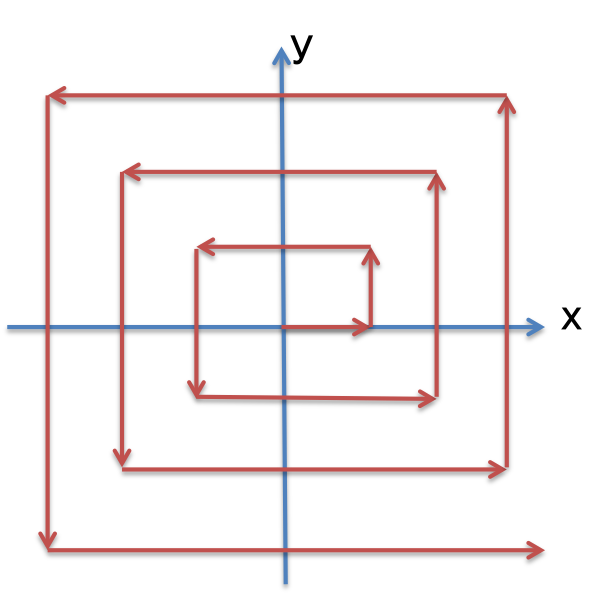
\includegraphics[clip,width=7.0cm]{fig1.png}
    \caption{}
    \label{fig:chokuseki}
  \end{center}
\end{figure}

\item
4と同様に、直積を順番に考え、今度は$(x,y)$の代わりに$\frac{x}{y}$として並べる。つまり\\
\[\frac{0}{0},\frac{1}{0},\frac{1}{1},\frac{0}{1},\frac{-1}{1},\frac{-1}{0},\frac{-1}{-1},\frac{0}{-1},
\frac{1}{-1},\frac{2}{-1},\frac{2}{0},\frac{2}{1},\frac{2}{2},\frac{1}{2},\frac{0}{2},\frac{-1}{2},\frac{-2}{2},\frac{-2}{1},\frac{-2}{0},\frac{-2}{-1},\frac{-2}{-2},\frac{-1}{-2},\frac{0}{-2},\dots\]
ここで、
\begin{enumerate}
\item 分母が0になっているものを削除。
\item 約分すると同じ値になるものは、後に出現しているものを削除。
\end{enumerate}
という操作をして、並べ直すと、
\[\frac{1}{1},\frac{0}{1},\frac{-1}{1},\frac{2}{-1},\frac{2}{1},\frac{1}{2},\frac{-1}{2},\dots\]
ここで、それぞれの分数の現れる順番と分数の値の関係は、自然数の集合から有理数全体の集合への全単射の写像になっている。よって、有理数全体の集合$\mathbb{Q}$は可算集合。
\item
ある集合$A$が可算集合とする。このとき、$A$の無限部分集合$X(X\subset A)$について考える。$A$は可算集合なので、自然数から$A$への全単射の写像$f:\mathbb{N}\to A$が存在する。ここで、$A$の集合を以下のように並べる。
\[f(1),f(2),f(3),f(4),\dots\]
さらに、この順番を保ちながら、$X$に含まれていない要素を取り除き、順番に番号を振る。この番号とそれぞれの要素の対応は、自然数の集合から$X$への全単射になっている。
\end{enumerate}

%%% 7.5
\subsection{}
$f:A\to\mathfrak{P}(A)$が全射とする。
\begin{equation}
X=\{b\in A|b\notin f(b)\} \tag{7.5.1}\\
\end{equation}
とすると、$X\in\mathfrak{P}(A)$かつ$f$が全射なので、$f(x)=X$となる$x\in A$が存在する。\\
もし、$x\in X$と仮定すると、$x$は$(7.5.1)$の条件を満たすはずなので、$x\notin X$となり、矛盾。\\
もし、$x\notin X$と仮定すると、$x$は$(7.5.1)$の条件を満たさないはずなので、$x\in f(x)$となり、矛盾。\\
いずれにしても矛盾するので、$f$は全射ではないことが示された。


%%%% 7.6
\subsection{}
$\mathfrak{P}(\mathbb{N})$を次のような三つの部分集合族$P_1, P_2, P_3$に分割する。$\mathbb{N}$の有限部分集合の全体を$P_1$、$\mathbb{N}$の部分集合で補集合が有限集合であるものの全体を$P_2$、それ以外の$\mathbb{N}$の部分集合の全体を$P_3$とする。$P_1,P_2およびP_1 \cup P_2$は加算集合である。実際、$f_1:\mathbb{N}\to P_1$を以下のように定義する。
\begin{align*}
f_1(1)&=\emptyset\\
f_1(2)&=\{1\}\\
f_1(3)&=\{2\}\\
f_1(4)&=\{1,2\}\\
f_1(5)&=\{3\}\\
f_1(6)&=\{1,3\}\\
f_1(7)&=\{2,3\}\\
f_1(8)&=\{1,2,3\}\\
f_1(9)&=\{4\}\\
\dots
\end{align*}
このとき、$f_1$は全単射になる。\\
また、$f_2:\mathbb{N}\to P_2$を$f_2(n)=\mathbb{N}-f_1(n)$と定義すれば、これは全単射になる。\\
さらに$g:\mathbb{N}\to P_1 \cup P_2$を
\[g(n)=
\begin{cases}
f_1(\frac{n}{2})  \qquad(nが偶数)\\
f_2(\frac{n+1}{2})  \quad(nが奇数)
\end{cases}
\]
と定義すれば、これは全単射になる。\\
$P_1\cup P_2 \sim \mathbb{N}$かつ、$P_2\sim \mathbb{N}$なので、$P_1\cup P_2\sim P_2$。$\mathfrak{P}(\mathbb{N})=P_1\cup P_2 \cup P_3$なので、結局、$\mathfrak{P}(\mathbb{N})\sim P_2 \cup P_3$。\\
また、$I=(0,1]$とすると、$\mathbb{R}\sim I$であることが6章の議論でわかるので、以下では、$P_2\cup P_3 \sim I$を証明する。\\

今、$x\in(0,1]$を$x=0.11010100\dots$のように2進数で表示することにする。ただし、$x=0.1$は$x=0.0\dot{1}$のように、必ず無限小数で表すことにする\footnote{任意の$x\in(0,1]$が、この無限小数の形式で一意に表現できることは、証明すべきことだと思う。ここでは省略する。}。\\
$h:(0,1]\to P_2\cup P_3$を以下のように定義する。\\
\[h(x)=\{n\in\mathbb{N}|xを2進数表示したときの小数第n位が1となる\}\]
$h$は全単射となるので、$P_2\cup P_3 \sim I$が示された\footnote{$h(x)$が無限集合なので、$P_1\cup P_2\cup P_3$でなく、$ P_2\cup P_3$を考える必要があった。}。結局、$\mathfrak{P}(\mathbb{N})\sim\mathbb{R}$が示された。

%%% 7.7
\subsection{}
\begin{enumerate}
\item
\[f:\mathbb{Z}\times(0,1]\to\mathbb{R}\]を\[f(x,y)=x+y\]と定義すれば、$f$は全単射である。よって、$\mathbb{N}\times\mathbb{R}\sim\mathbb{Z}\times(0,1]\sim\mathbb{R}$。

\item
$\frak{P}(A)\sim F(A,\{0,1\})$である。実際、任意の$X\in\frak{P}(A)$に対して、
\[f_X(x)=
\begin{cases}
1 \quad(x\in X)\\
0 \quad(x\notin X)
\end{cases}
\]
と定義される$f_X\in F(A,\{0,1\})$を対応させればこれは全単射になる。よって、$\frak{P}(A)\sim F(A,\{0,1\})$がわかる。\\
また、問7.2により、$F(A\times B,C)\sim F(A,F(B,C))$である。以上より、
\begin{align*}
F(\mathbb{R},\mathbb{R})&\sim F(\mathbb{R},\frak{P}(\mathbb{N}))\\
&\sim F(\mathbb{R},F(\mathbb{N},\{0,1\}))\\
&\sim F(\mathbb{R}\times\mathbb{N},\{0,1\})\\
&\sim F(\mathbb{R},\{0,1\})\\
&\sim \frak{P}(\mathbb{R})
\end{align*}
\end{enumerate}

%%%7.8
\subsection{}
実数値連続関数$f_1,f_2$が任意の$x\in\mathbb{Q}$で$f_1(x)=f_2(x)$ならば、$f_1$と$f_2$は同一である。よって、実数値連続関数全体の集合と$F(\mathbb{Q},\mathbb{R})$は濃度が等しい。\\
問7.4より、$\mathbb{Q}\sim\mathbb{N}$かつ$\mathbb{N}\times\mathbb{N}\sim\mathbb{N}$なので、$\mathbb{Q}\times\mathbb{N}\sim\mathbb{N}$である。
\begin{align*}
F(\mathbb{Q},\mathbb{R})&\sim F(\mathbb{Q}, \frak{P}(\mathbb{N}))\\
&\sim F(\mathbb{Q},F(\mathbb{N},\{0,1\}))\\
&\sim F(\mathbb{Q}\times\mathbb{N}, \{0,1\})\\
&\sim F(\mathbb{N},\{0,1\})\\
&\sim \frak{P}(\mathbb{N})\\
&\sim \mathbb{R}
\end{align*}

%%% 7.9
\subsection{}
整数係数の多項式\[f(x)=a_0+a_1x+a_2x^2+\dots+a_nx^n\quad(n\geq 1, a_n\neq0)\]に対して、\[H(f)=n+|a_0|+|a_1|+\dots+|a_n|\]とおく。$H(f)$は2以上の自然数である。今、自然数$h\geq2$に対して、整数係数の多項式の集合$F_h$を
\[F_h=\{f|H(f)=h\}\]
と定義する。$F_h$は有限集合である。また、n次多項式の根は高々n個なので、$F_h$に属する多項式の根となるような複素数の集合も有限集合である。つまり、$h\geq 2$に対して、$F_h$に属する多項式の根を一列に並べることができる\footnote{たとえば、複素数の実部で昇順に並べて、そのあと虚部で昇順に並べるなどの方法が考えられる}。以上の議論より、任意の代数的数に対して、自然数$n\in\mathbb{N}$を対応させる全単射の写像を作ることができることがわかる。よって、代数的数全体の集合は可算集合である。


%%%7.10
\subsection{}
$z$を整数係数の多項式$f(x)$の根とする。よって、
\[f(z)=0\]
$p$を自然数とすれば\[f(px)=a_0+a_1px+a_2p^2x^2+\dots+a_np^nx^n\]は整数係数の多項式になり、$\frac{z}{p}$は$f(px)$の根である。
したがって、$\alpha$をある超越数とすれば、全ての自然数$p$に対して$p\alpha$も超越数であることがわかる\footnote{$p\alpha$が超越数でない、つまり代数的数であると仮定すると、$\alpha$も代数的数であることになってしまい矛盾。}。代数的数であるような実数の全体は可算集合であり、実数全体の集合$\mathbb{R}$は非可算であるから、超越数の存在がわかる。その一つを$\alpha$とする。$\mathbb{R}$を次のような三つの部分集合$A_1,A_2,A_3$に分割する。代数的数であるような実数の全体を$A_1$とする。\[A_2=\{p\alpha|p\in \mathbb{N}\}\]とする。$A_1,A_2$に属さない実数の全体を$A_3$とする。\\
$A_2\cup A_3$は超越数全体の集合である。$A_1$は問7.9で証明したように加算集合である。
\[g_1(n)=\alpha n\]
という関数$g_1:\mathbb{N}\to A_2$が全単射になるので、$A_2$は加算集合である。$g_2:\mathbb{N}\to A_1$を全単射の写像とすると、
\[h(n)=
\begin{cases}
g_1(\frac{n+1}{2})\quad(nが奇数)\\
g_2(\frac{n}{2})\qquad(nが偶数)\\
\end{cases}
\]
という写像$h:\mathbb{N}\to A_1\cup A_2$が全単射になるので、$A_1\cup A_2$も可算集合である。特に、$A_1\cup A_2\sim A_2$となる。よって、$\mathbb{R}=A_1\cup A_2\cup A_3\sim A_2\cup A_3$。

%%% section 8
\section{二項関係}

%%% 8.1
\subsection{}
\begin{enumerate}
\item $G(\rho_1)=\{(x,y)|x\geq0,y\geq0\}$について
\begin{enumerate}
\item 反射律 満たさない\\
$x=-1$のとき、$x\rho_1 x$を満たさない。
\item 対称律 満たす\\
$x\geq0,y\geq0$ならば、$y\geq0,x\geq0$である。
\item 推移律 満たす\\
$x\geq0,y\geq0$かつ$y\geq0,z\geq0$ならば$x\geq0,z\geq0$である。
\item 反対称律 満たさない\\
$x=1,y=2$のとき、$x\geq 0,y\geq0$かつ$y\geq0,x\geq0$だが、$x\neq y$。
\end{enumerate}

\item $G(\rho_2)=\{(x,y)|x\leq y\}$について
\begin{enumerate}
\item 反射律 満たす\\
$x\leq x$である。
\item 対称律 満たさない\\
$x=1,y=2$のとき、$x\leq y$だが、$y\leq x$でない。
\item 推移律 満たす\\
$x\leq y$かつ$y\leq z$ならば、$x\leq z$。
\item 反対称律 満たす\\
$x\leq y$かつ$y\leq x$ならば$x=y$である。
\end{enumerate}

\item $G(\rho_3)=\{(x,y)|(x-y)(x+y-1)=0\}$について\\
$f(x,y)=(x-y)(x+y-1)$とおく。
\begin{enumerate}
\item 反射律 満たす\\
$x-x=0$なので$f(x,x)=0$である。
\item 対称律 満たす\\
$f(x,y)=0$のとき、$f(y,x)=(y-x)(y+x-1)=-f(x,y)=0$。
\item 推移律 満たす\\
$f(x,y)=0$と$f(y,z)=0$を仮定する。
\begin{enumerate}
\item $x-y=0,y-z=0$のとき\\
$x-z=0$となるので、$f(x,z)=0$。
\item $x-y=0, y+z-1=0$のとき\\
$x+z-1=0$となるので、$f(x,z)=0$。
\item $x+y-1=0, y-z=0$のとき\\
$x+z-1=0$とのあるので、$f(x,z)=0$。
\item $x+y-1=0, y+z-1=0$のとき\\
$x-z=0$となるので、$f(x,z)=0$。
\end{enumerate}
\item 反対称律 満たさない\\
$x=0.7,y=0.3$のとき、$f(x,y)=0$かつ$f(y,x)=0$だが、$x\neq y$。
\end{enumerate}

\item $G(\rho_4)=\{(x,y)|(x-y)(x-y+1)(x-y-1)=0\}$について\\
$g(x,y)=(x-y)(x-y+1)(x-y-1)$とおく。
\begin{enumerate}
\item 反射律 満たす\\
$x-x=0$なので$g(x,x)=0$。
\item 対称律 満たす\\
$g(x,y)=0$のとき、$g(y,x)=(y-x)\{(y-x)^2-1\}=-g(x,y)=0$。
\item 推移律 満たさない\\
$x=2,y=1,z=0$のとき、$g(x,y)=0$かつ$g(y,z)=0$だが、$g(x,z)\neq 0$。
\item 反対称律 満たさない\\
$x=2,y=1$のとき、$g(x,y)=0$かつ$g(y,x)=0$だが、$x\neq y$。
\end{enumerate}
\end{enumerate}

\subsection{}
定義より、$A\rho B\Longleftrightarrow (A-B)\cup(B-A)が有限集合$。
\begin{enumerate}
\item 反射律\\
$A-A=\emptyset$なので、$A\rho A$。
\item 対称律\\
$(A-B)\cup(B-A)=(B-A)\cup(A-B)$なので、$A\rho B$ならば$B\rho A$。
\item 推移律\\
$(A-B)\cup(B-A)=X,(B-C)\cup(C-B)=Y$が有限集合とする。
\begin{align*}
(A-C)\cup(C-A)&=\{x|(x\in A かつ x\notin C)または(x\in Cかつx\notin A)\}\\
&=\{x|(x\in A かつ x\in B かつ x\notin C)または(x\in A かつ x\notin Bかつx\notin C)または\\
&\qquad\qquad(x\in Cかつx\in Bかつx\notin A)または(x\in Cかつx\notin Bかつx\notin A)\}\\
&\subset\{x|(x\in B かつ x\notin C)または(x\in A かつ x\notin B)または\\
&\qquad\qquad(x\in Bかつx\notin A)または(x\in Cかつx\notin B)\}\\
&=\{x|x\in X またはx\in Y\}\\
&=X\cup Y
\end{align*}
よって、$(A-C)\cup(C-A)$も有限集合
\end{enumerate}


%%%8.3
\subsection{}
\begin{enumerate}
\item 反射律
\[\forall x\in X[f(x)=f(x)]\]
\item 対称律
\[\forall x,y\in X[f(x)=f(y)\Longrightarrow f(y)=f(x)]\]
\item 推移律
\[\forall x,y,z\in X[f(x)=f(y) かつf(y)=f(z)\Longrightarrow f(x)=f(z)]\]
\end{enumerate}
よって、$G(\rho)$は反射律、対称律、推移律を満たす。\\
今、$C(x)=\{a\in X|f(a)=f(x)\}$なので、$\forall a\in C(x)[f(a)=f(x)]$。よって、$g(C(x))=f(x)$とすれば、関数$g:X/\rho\to Y_1$が一意に定義できる。\\
$g$は全射である。実際、$f(X)=\{f(x)\in Y|x\in X\}=Y_1$だから、任意の$y\in Y_1$に対して、$f(x)=y$となる$x$が存在する。よって、任意の$y\in Y_1$に対して、$g(C(x))=y$となる$C(x)\neq\emptyset$が存在する。\\
$g$は単射である。実際、$g(A)=g(B)=f(x)$とすると、$x\in Aかつx\in B$となる。$A$と$B$が交わっているので、$A=B$。

%%%8.4
\subsection{}
図\ref{fig:8.4.1}、図\ref{fig:8.4.2}、図\ref{fig:8.4.3}、図\ref{fig:8.4.4}がそれぞれ答え。
\begin{figure}[htbp]
  \begin{center}
    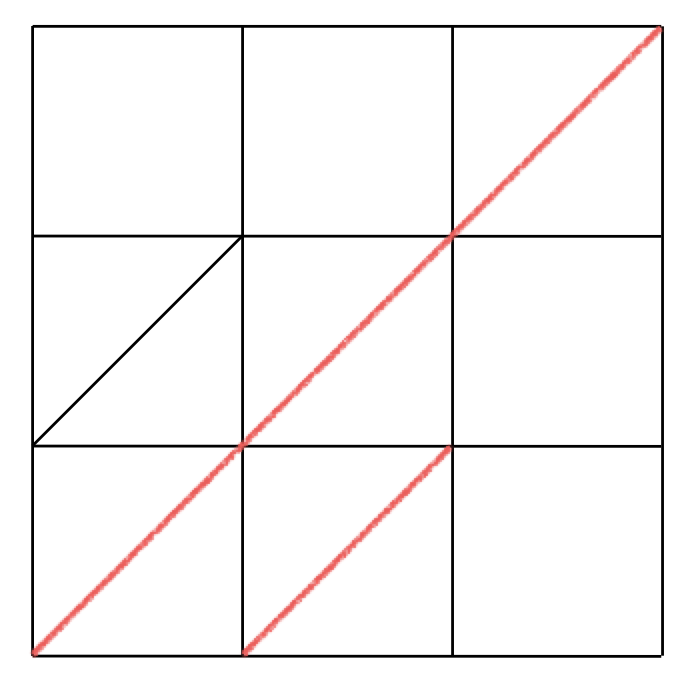
\includegraphics[clip,width=4.0cm]{8_4/8_4_1.png}
    \caption{反射律と対称律を満足するもの}
    \label{fig:8.4.1}
  \end{center}
\end{figure}

\begin{figure}[htbp]
  \begin{center}
    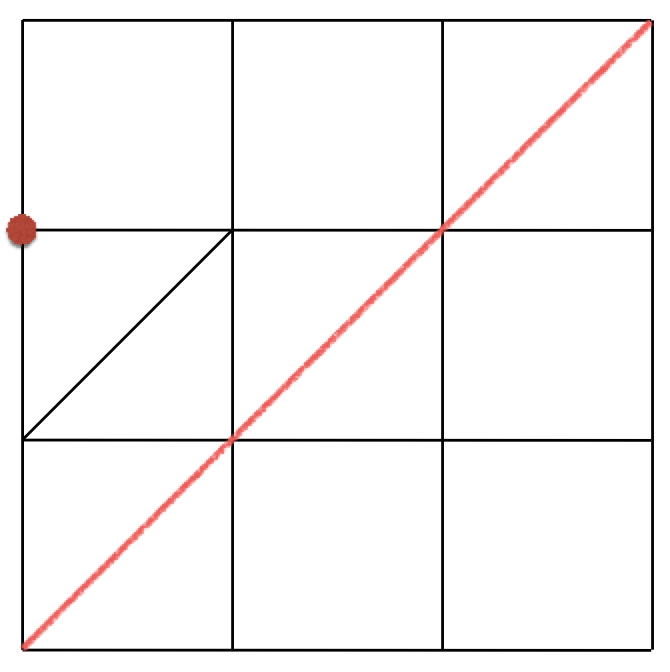
\includegraphics[clip,width=4.0cm]{8_4/8_4_2.png}
    \caption{反射律と推移律を満足するもの}
    \label{fig:8.4.2}
  \end{center}
\end{figure}
\begin{figure}[htbp]
  \begin{center}
    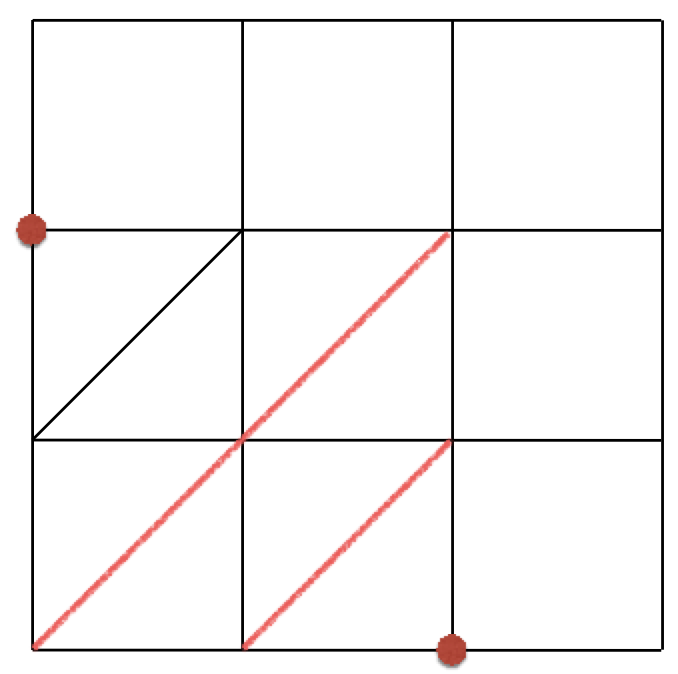
\includegraphics[clip,width=4.0cm]{8_4/8_4_3.png}
    \caption{対称律と推移律を満足するもの}
    \label{fig:8.4.3}
  \end{center}
\end{figure}\begin{figure}[htbp]
  \begin{center}
    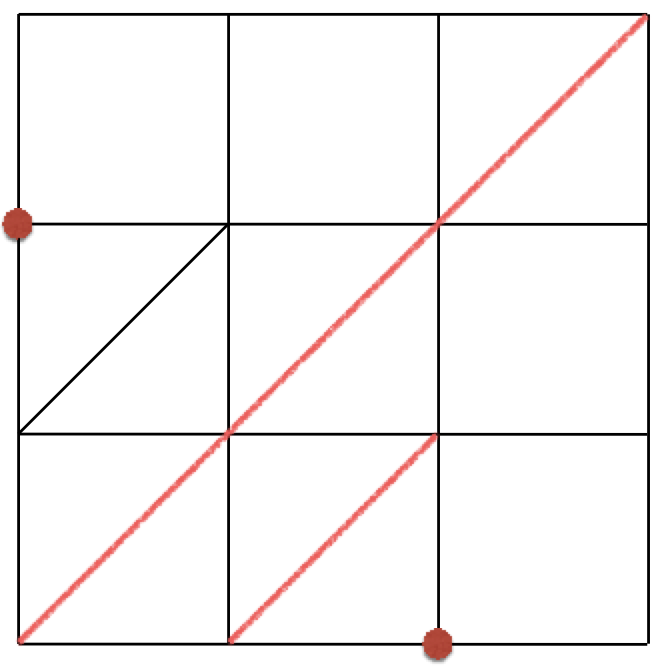
\includegraphics[clip,width=4.0cm]{8_4/8_4_4.png}
    \caption{同値関係であるもの}
    \label{fig:8.4.4}
  \end{center}
\end{figure}

\newpage

%%%8.5
\subsection{}
$\mathfrak{P}(A)$の任意の部分集合$\mathfrak{U}$に対して、
\[\inf \mathfrak{U}=\bigcap(E|E\in\mathfrak{U})\]
\[\sup \mathfrak{U}=\bigcup(E|E\in\mathfrak{U})\]
と定義すれば、確かに
\[\forall B\in \mathfrak{U}[\inf \mathfrak{U}\subset B]\]
\[\forall B\in \mathfrak{U}[B\subset \sup \mathfrak{U}]\]
が成り立つ。

%%% 8.6
\subsection{}
5元束と6元束については、巻末の解答を参照。7元束は図\ref{fig:8_6}のように53種類考えられる\footnote{点の色に特別に意味はない。場合分けの際にわかりやすくするために色付けした。}。
\begin{figure}[htbp]
  \begin{center}
    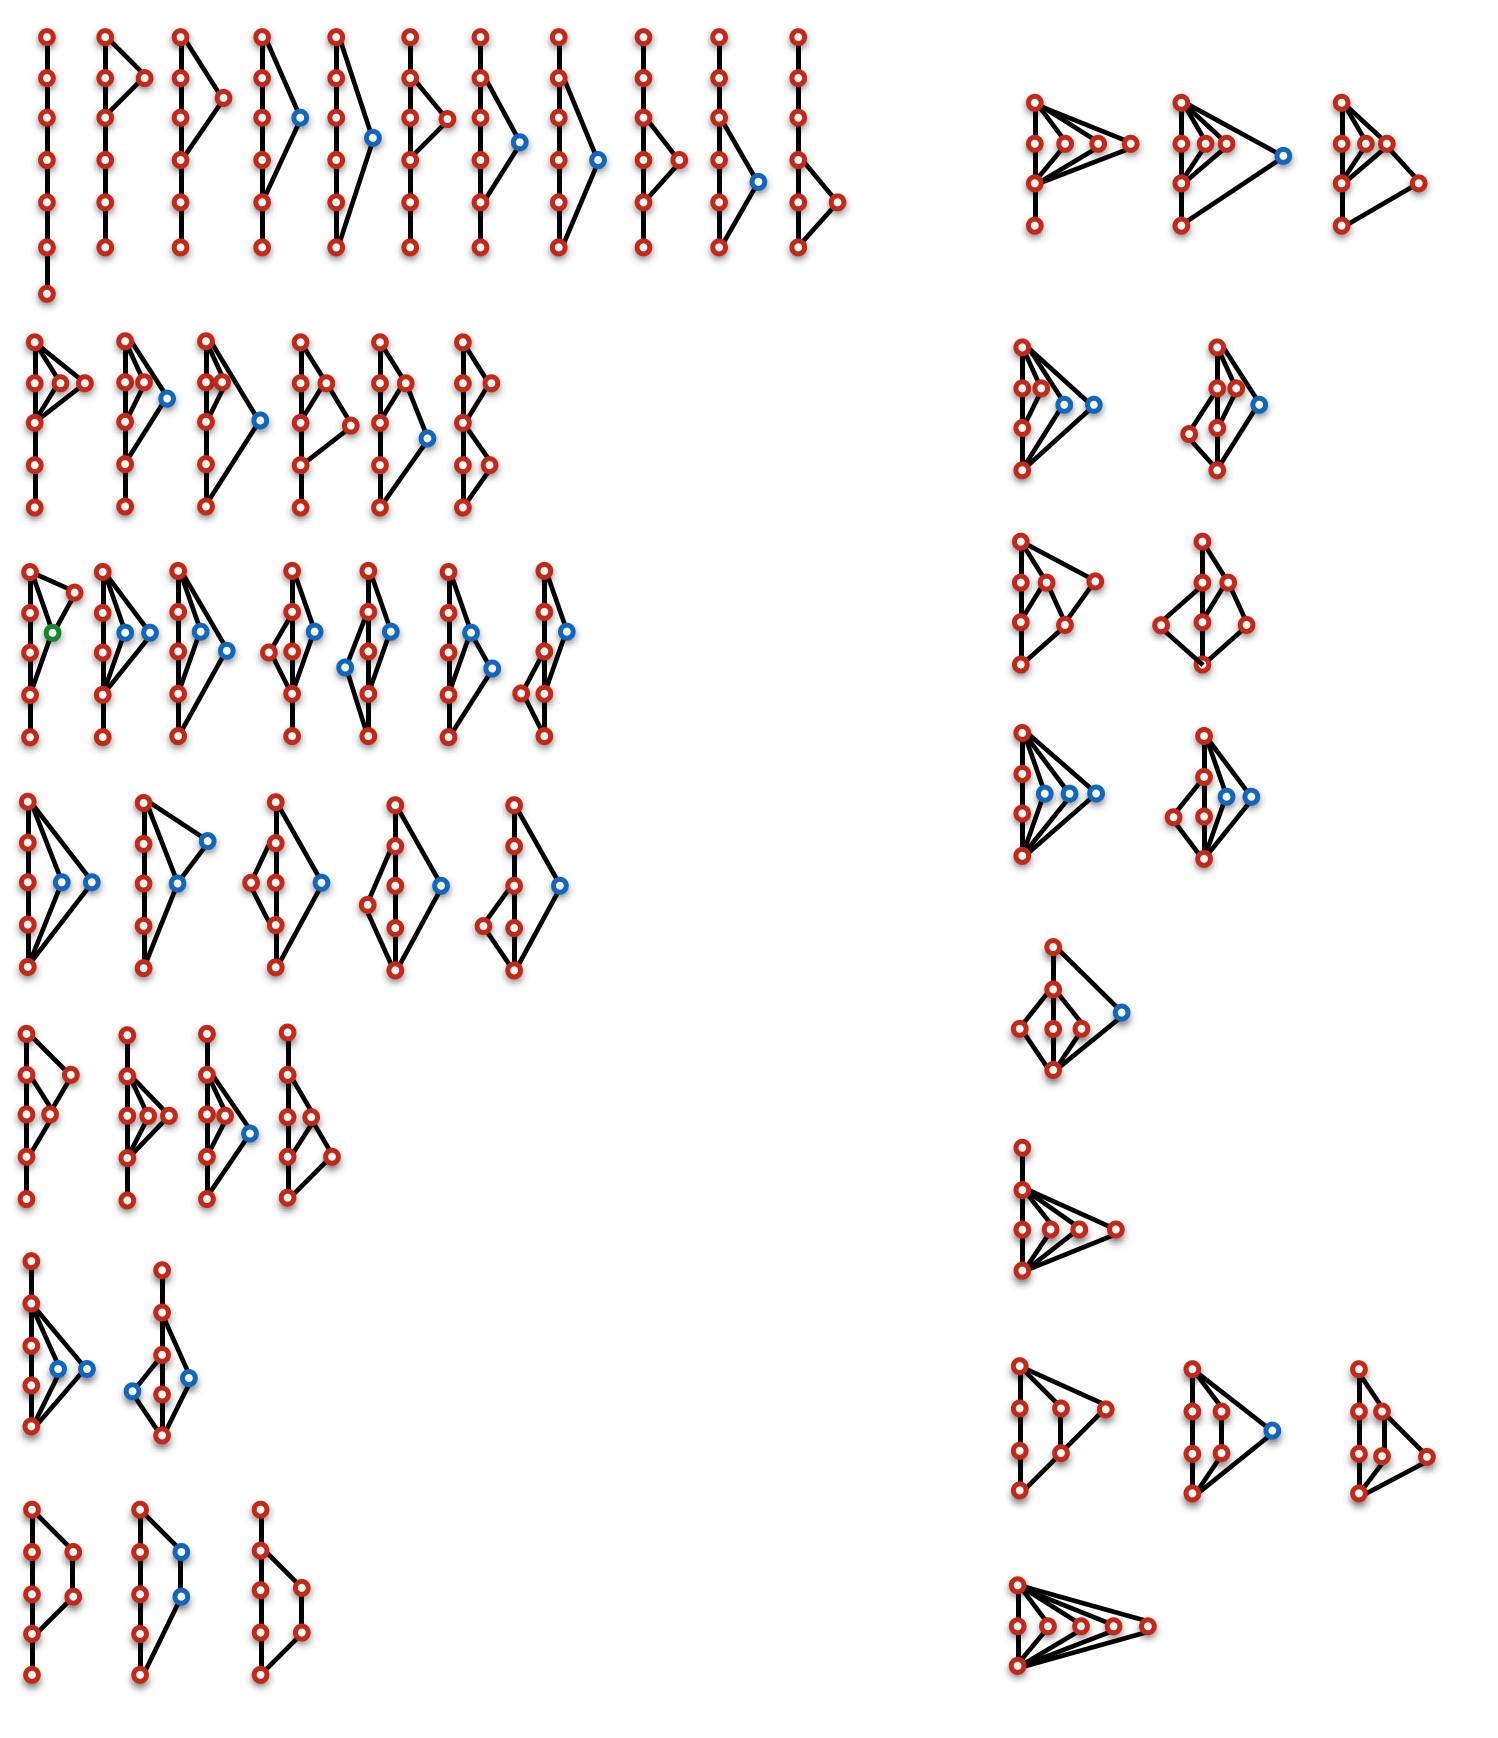
\includegraphics[clip,width=13.0cm]{8_6.png}
    \caption{7元束}
    \label{fig:8_6}
  \end{center}
\end{figure}

\newpage
%%%8.7
\subsection{}
$\mathfrak{U}=\{A\in X|A\subset\varphi(A)\}$とする。$\emptyset\subset\varphi(\emptyset)$なので、$\mathfrak{U}$は空集合にはならない。$E_0=\bigcup (A|A\in\mathfrak{U})$とおけば、$\forall A\in\mathfrak{U}[A\subset\varphi(A)\subset\varphi(E_0)]$なので、$E_0\subset\varphi(E_0)$である。$E_0\subsetneq\varphi(E_0)$とすると、$\varphi(E_0)\in\mathfrak{U}$であることに矛盾。よって、$E_0=\varphi(E_0)$である。


%%% section9
\part{整列集合と選択公理}
\section{整列集合}

%%%9.1
\subsection{}
\begin{align*}
(X\langle a\rangle)\langle b\rangle&=\{x\in X\langle a\rangle|x<b\}\\
&=\{x\in X| x\in X\langle a\rangle かつ x<b\}\\
&=\{x\in X| x<aかつx<b\}\\
&=\{x\in X|x<b\}\\
&=X\langle b\rangle
\end{align*}
ここで、$b<a$という前提により、「$x<aかつx<b\Longleftrightarrow x<b$」という関係を用いた。実際、$x<b$であって、$a\leq x$と仮定すると、$a\leq b$となり矛盾してしまう。

\subsection{}
\subsubsection{整列集合は、そのいかなる切片とも順序同型にならない}
\label{9_2}
ある切片$a\in X$に対して、$(X,\leq)\simeq(X\langle a\rangle,\leq)$が成り立つと仮定すると、順序を保つ全単射$f:X\to X\langle a\rangle$が存在することになる。$f$は単射なので、定理9.1により
\[\forall x\in X[x\leq f(x)]\]
が成り立つはずである。しかし、$f(a)\in X\langle a\rangle$なので、$f(a)<a$となってしまい矛盾。結局、$(X,\leq)\simeq(X\langle a\rangle,\leq)$ではないことがわかる。
\subsubsection{整列集合の相異なる二つの切片は互いに順序同型にならない}
整列集合の部分集合は整列集合である。今、$Y$を整列集合とし、$a,b (a<b, a\in Y, b\in Y)$に対して、
\[X= Y\langle b\rangle\]
とおくと、
\begin{align*}
X\langle a\rangle&=\{x\in X|x<a\}\\
&=\{x\in Y\langle b\rangle| x<a\}\\
&=\{x\in Y| x<aかつx<b\}\\
&=\{x\in Y|x<a\}\\
&=Y\langle a\rangle
\end{align*}
となり、$X\langle a\rangle=Y\langle a\rangle$が成り立つ。すると、\ref{9_2}と同様に、$(Y\langle a\rangle,\leq)\simeq(Y\langle b\rangle,\leq)$にはならないことが証明できる。

\subsection{}
$(A,\leq)$および$(B,\leq)$を整列集合とし、$f:A\to B$を順序同型写像とする。今、$f$は全単射なので、
\[x<y\Longleftrightarrow f(x)<f(y)\]
が成り立つ\footnote{左から右へは、$f$が順序を保ちかつ単射であることから証明できる。右から左へは、$f$が全射であることと、逆写像$f^{-1}$が存在することから証明できる。}。よって、任意の$a\in A$に対して、
\begin{align*}
f(A\langle a\rangle)&=\{f(x)\in B| x\in A\langle a\rangle\}\\
&=\{f(x)\in B|x<a かつ x\in A\}\\
&=\{f(x)\in B|f(x)<f(a) かつ x\in A\}\\
&=\{y\in B|y<f(a)\}\\
&=B\langle f(a)\rangle
\end{align*}

%%%% 9.4
\subsection{}
以下では、$\varphi:X_1\to Y_1$が順序同型写像であることを証明するため、$\varphi$が全単射の写像であることと、$\varphi$が順序を保つ写像であることを証明する。定義より、$X_1,Y_1$はそれぞれ、
\[X_1=\{a\in X|\exists b\in Y[X\langle a\rangle\simeq Y\langle b\rangle]\}\]
\[Y_1=\{b\in Y|\exists a\in X[X\langle a\rangle\simeq Y\langle b\rangle]\}\]
このとき、各元$a\in X_1$に対して、$X\langle a\rangle\simeq Y\langle b\rangle$となる$b\in Y_1$がただ一つ存在する。実際、$b_1,b_2\in Y_1$が$X\langle a\rangle\simeq Y\langle b_1\rangle$かつ$X\langle a\rangle\simeq Y\langle b_2\rangle$となると仮定すると、$Y\langle b_1\rangle\simeq Y\langle b_2\rangle$であり、順序同型写像$f:Y\langle b_1\rangle\to Y\langle b_2\rangle$が存在する。$b_1<b_2$と仮定すると、順序を保つ単射$f$に対して、$f(b_1)<b_2$となり、定理9.1に矛盾する。$b_1>b_2$としてもやはり矛盾が生じるので、$b_1=b_2$になるはずである。結局、$X\langle a\rangle\simeq Y\langle b\rangle$となる$b$がただ一つ存在することがわかった。さて、以上の議論を逆に$b$を中心に展開すると、任意の$b\in Y_1$に対して、$X\langle a\rangle\simeq Y\langle b\rangle$となる$a$がただ一つ存在することになる。よって、$b=\varphi(a)$と定義される写像$\varphi$は全単射である。\\
 $a_1,a_2\in X_1$が$a_1\leq a_2$であると仮定する。$X\langle a_1\rangle\simeq Y\langle \varphi(a_1)\rangle$の順序同型写像$\psi_1$
\[\psi_1:Y\langle \varphi(a_1)\rangle\to X\langle a_1\rangle\]
は順序を保つ全単射の写像である。また、$X\langle a_2\rangle\simeq Y\langle \varphi(a_2)\rangle$の順序同型写像$\psi_2$
\[\psi_2:X\langle a_2\rangle\to Y\langle \varphi(a_2)\rangle\]
も順序を保つ全単射の写像である。よって、$\psi=\psi_2\circ\psi_1$
\[\psi:Y\langle \varphi(a_1)\rangle\to Y\langle \varphi(a_2)\rangle\]
は順序を保つ単射の写像である\footnote{$X\langle a_1\rangle\subset X\langle a_2\rangle$なので$\psi$は全射とは限らない。}ので、定理9.1より、$\varphi(a_1)\leq\varphi(a_2)$である\footnote{$\varphi(a_1)>\varphi(a_2)$と仮定すると、$\psi(\varphi(a_2))<\varphi(a_2)$となり、定理9.1に反する}。結局\[a_1\leq a_2\Longleftrightarrow\varphi(a_1)\leq\varphi(a_2)\]となり、$\varphi$が順序を保つ写像であることが証明できた。\\
 以上より、$\varphi:X_1\to Y_1$は順序同型写像である。

\subsection{}
(1)と(2)が同時に成り立つと仮定し、順序同型$X\simeq Y, X\simeq Y\langle b\rangle$が成り立つとする。すると、$Y\simeq Y\langle b\rangle$が成り立つ。$Y\simeq Y\langle b\rangle$の順序同型写像を$f:Y\to Y\langle b\rangle$とすると、$f(b)<b$となり、定理9.1に矛盾する。従って、(1)と(2)は同時には成り立たない。\\
 (1)と(3)が同時に成り立たないことも同様に証明できる。

\section{選択公理}
\subsection{}
$f$を集合$A$の上の一つの選択関数とする。$f$は$A$の空でない部分集合の全体$\mathfrak{U}=\mathfrak{P}(A)-\{\emptyset\}$から、$A$への写像であり、$f(B)\in B\subset A$である。$m<n$と仮定すると
\[a_n=f(A-\{a_1,\dots,a_m,\dots,a_{n-1}\})\]
となり、$a_m\notin A-\{a_1,\dots,a_m,\dots,a_{n-1}\}$なので、$a_m\neq a_n$。$n<m$の場合も同様に証明できる。

\subsection{}	
$W_\infty$の一つの上界が$W_\infty$に含まれるならば、それは$W_\infty$の最大限になる。以下では、$w\in W_\infty$であることを背理法で証明する。\\
 $w\notin W_\infty$と仮定し、
\[\Delta_\infty=\{x\in X| a\in W_\infty ならば a<x\}\]
とおく。$w\notin W_\infty$であり、$w$が$W_\infty$の上界であることから$w\in \Delta_\infty$。よって$\Delta_\infty\neq\emptyset$である。そこで、$z=f(\Delta_\infty)$とおく。このとき、$W_*=W_\infty\cup\{z\}$は整列集合である。
$W_\infty=W_*\langle z\rangle$であるから、$\Delta_\infty=\Delta(W_*,z)$であり、$W_*$も$f$-列になる\footnote{
\begin{enumerate}
\item
$a\in W_\infty$のとき、
\begin{align*}
\Delta(W_*, a)&=\{x\in X|b\in W_*\langle a\rangle ならば b<x\}\\
&=\{x\in X|b\in W_\infty\langle a\rangle ならば b<x\}\\
&=\Delta(W_\infty, a)
\end{align*}
なので、$f(\Delta(W_*, a))=f(\Delta(W_\infty, a))=f(a)$である。
\item
$a=z$のとき、
\begin{align*}
\Delta(W_*, z)&=\{x\in X|b\in W_*\langle z\rangle ならば b<x\}\\
&=\{x\in X|b\in W_\infty ならば b<x\}\\
&=\Delta_\infty
\end{align*}
なので、$f(\Delta(W_*, z))=f(\Delta_\infty)=z$である。
\end{enumerate}
}。

これは$W_\infty$が最大$f$-列であることに矛盾する。したがって、$w\in W_\infty$であることがわかった。よって、$w$は$W_\infty$の最大限である。


%%%%%  section 11  %%%%%%%%%%%
\section{整列可能定理}
\subsection{}
\subsubsection{}
\label{11_1_1}
$W=\bigcup(W_\lambda|\lambda\in\Lambda)$の2元$x,y$に対して、
\[x\in W_\lambda,\quad y\in W_\lambda\]
となる元$\lambda\in\Lambda$が存在しないと仮定する。すると、ある$\lambda_1,\lambda_2\in\Lambda$に対して
\[\lambda_1\neq\lambda_2\]
\[x\in W_{\lambda_1},\quad x\notin W_{\lambda_2},\quad y\in W_{\lambda_2},\quad y\notin W_{\lambda_1}\]
が成り立つことになる。これは「$\Lambda$の異なる2元$\alpha,\beta$に対しては、常に$(W_\alpha,\leq_\alpha),(W_\beta,\leq_\beta)$の中のいずれか一方は他方の切片になっている」という仮定に反する。

\subsubsection{}
\label{11_1_2}
「$\Lambda$の異なる2元$\alpha,\beta$に対しては、常に$(W_\alpha,\leq_\alpha),(W_\beta,\leq_\beta)$の中のいずれか一方は他方の切片になっている」という仮定により、ある$\lambda\in\Lambda$に対して、
$x,y\in W_\lambda かつ x\leq_\lambda y$
が成り立つならば、任意の$\lambda'\in\Lambda$に対しても、
\[x,y\in W_{\lambda'}\Longrightarrow x\leq_{\lambda'}y\]
が成り立つ。

\subsubsection{}
$W$の上の二項関係$\leq$は順序関係であることを証明する。
\begin{enumerate}
\item{反射律}\\
$\forall\lambda\in\Lambda[x\in W_\lambda\Longrightarrow x\leq_\lambda x]$なので、$\forall x\in W[x\leq x]$が成り立つ。

\item{推移律}\\
\ref{11_1_1}と同様の議論により、任意の3元$x,y,z\in W$に対して
\[x\in W_\lambda,\quad y\in W_\lambda,\quad z\in W_\lambda\]
となる元$\lambda\in\Lambda$が存在することがわかる。$\leq_\lambda$が順序関係なので、
\[x\leq_\lambda y かつ y\leq_\lambda z ならば x\leq_\lambda z\]
が成り立つ。よって、$\leq$も
\[x\leq y かつ y\leq z ならば x\leq z\]
が成り立つ。

\item{反対称律}\\
\ref{11_1_1}により、任意の2元$x,y\in W$に対して
\[x\in W_\lambda,\quad y\in W_\lambda\]
となる元$\lambda\in\Lambda$が存在する。$\leq_\lambda$が順序関係なので、
\[x\leq_\lambda y かつ y\leq_\lambda x ならば x=y\]
が成り立つ。よって、$\leq$も
\[x\leq y かつ y\leq x ならば x=y\]
が成り立つ。\\
\end{enumerate}
以上より、$W$の上の二項関係$\leq$は順序関係であることがわかった。\\

$W$は整列集合になることを証明する。\\
$W$の空でない部分集合を$U$とする。$U$の元$x$に対して、$x\in W_\lambda$となる$\lambda\in\Lambda$が存在する。$W_\lambda$は整列集合なので、$W_\lambda\cap U$には最小値$y=\min(W_\lambda\cap U)$が存在する。この$y$は$U$の最小値でもある。実際、もしも$z<y$となる$z\in U$が存在すると仮定すると、$z<y$にも関わらず、$z\notin W_\lambda$ かつ $y\in W_\lambda$となってしまう。$z\in W$なので、$z\in W_{\lambda'}$という$\lambda'\in\Lambda$が存在するはずだが、これは「$\Lambda$の異なる2元$\alpha,\beta$に対しては、常に$(W_\alpha,\leq_\alpha),(W_\beta,\leq_\beta)$の中のいずれか一方は他方の切片になっている」という仮定に矛盾する。結局、$y=\min(W_\lambda\cap U)$は$U$の最小値でもある。半順序集合$(W,\leq)$の任意の部分集合$U$に対して最小値が存在するので、$W$は整列集合である。


\subsubsection{}
\ref{11_1_2}により、$\forall\lambda\in\Lambda$に対して、\[x\leq_\lambda y\Longrightarrow x\leq y\]が成り立つ。
また、定義より$\forall \lambda\in\Lambda[W_\lambda\subset W]$が成り立つ。よって、「各$\lambda\in\Lambda$に対して、$(W_\lambda,\leq_\lambda)$は$(W,\leq)$に一致するかまたは$(W,\leq)$の切片になる」ということを証明するためには、
\[\forall x\in W-W_\lambda[\forall y\in W_\lambda[y<x]]\]
が成り立つことを証明すればよい。ある$x\in W-W_\lambda$に対して、$x\leq y$となる$y\in W_\lambda$が存在すると仮定すると、$x\leq y$にも関わらず、$x\notin W_\lambda$かつ$y\in W_\lambda$となってしまい、「$\Lambda$の異なる2元$\alpha,\beta$に対しては、常に$(W_\alpha,\leq_\alpha),(W_\beta,\leq_\beta)$の中のいずれか一方は他方の切片になっている」という仮定に矛盾する。以上より、各$\lambda\in\Lambda$に対して、$(W_\lambda,\leq_\lambda)$は$(W,\leq)$に一致するかまたは$(W,\leq)$の切片になっている。

\subsection{}
\subsubsection{例11.1}
$A$の部分集合$W$と単射の関数$f:W\to B$の組$(W,f)$全体の集合を$\mathfrak{U}$とおく。$\mathfrak{U}$は空ではない。実際、$A$の一つの元$a$だけからなる集合$W=\{a\}$から$B$への写像$f:\{a\}\to B$は単射である。$\mathfrak{U}$の元$(W,f),(W',f')$に対して、$(W,f)\leq (W',f')$を以下のように定義する。
\[ W\subset W' かつ \forall x\in W[f(x)=f'(x)]\]
このとき、$(\mathfrak{U},\leq)$は帰納的半順序集合になる。実際、半順序集合になることは反射律、推移律、反対称律を確かめることでわかる。また、全順序部分集合$\mathfrak{W}$に対して、\[X=\bigcup_{(W,f_W)\in \mathfrak{W}}W\]と$X$を定義する。さらに、$f_X:X\to B$を、$x\in W$となる$(W,f_W)\in\mathfrak{W}$が存在するときに$f_X(x)=f_W(x)$と定義する。$\mathfrak{W}$が全順序集合であることから、$f_X$は一意に定義されている。
このとき、$(X,f_X)$は$\mathfrak{W}$の上界になる。実際、任意の$(W,f_W)\in\mathfrak{W}$に対して、$W\subset X$と、$\forall x\in W[f_W(x)=f_X(x)]$が成り立つので、任意の$(W,f_W)\in\mathfrak{W}$に対して$(W,f_W)\leq (X,f_X)$が成り立つ。結局、$(X,f_X)$は$\mathfrak{W}$の上界である。\\
ツォルンの補題により帰納的半順序集合は極大元を持つので、$(W,f)\in\mathfrak{U}$を一つの極大元とすれば、$W=A$または$f(W)=B$のいずれかが成り立つ。$W=A$のときは$A$から$B$への単射が存在し、$f(W)=B$のときは$B$から$A$への単射が存在する。

\subsubsection{例11.2}
$\mathbb{R}$の部分集合$B$は、$B$に属する有限個の実数が常に$\mathbb{Q}$上一次独立であるとき、$\mathbb{Q}$上一次独立な集合という。$\mathbb{Q}$上一次独立な集合の全体を$\mathfrak{B}$とする。$\mathfrak{B}$は空でない。実際、たとえば$\{1\}$は$\mathbb{Q}$上一次独立な集合である。$X,Y\in\mathfrak{B}$に対して、$X\leq Y$を以下のように定義する。
\[X\leq Y\Longleftrightarrow X\subset Y\]
このとき、$(\mathfrak{B},\leq)$は帰納的半順序集合になる。実際、全順序部分集合$\mathfrak{A}$に対して、
\[U=\bigcup_{X\in\mathfrak{A}}X\]
とおけば、$U\in\mathfrak{B}$であり\footnote{$\mathfrak{A}$は全順序部分集合なので、任意の実数$x_1,x_2,\dots,x_r\in U$に対して、ある$X\in\mathfrak{A}$が存在し、$x_1,x_2,\dots,x_r\in X$となるはずである。$X$は$\mathbb{Q}$上一次独立な集合なので、$x_1,x_2,\dots,x_r$は一次独立であり、$U\in\mathfrak{B}$であることがわかる。}、任意の$X\in\mathfrak{A}$に対して、$X\subset U$、つまり$X\leq U$が成り立ち、$U$は上界になっている。よって、任意の全順序部分集合に対して上界が存在するので、$(\mathfrak{B},\leq)$は帰納的半順序集合になっている。$B$を$\mathfrak{B}$の一つの極大元とする。すなわち$B$は$\mathbb{Q}$上一次独立な極大集合である。このとき、任意の実数は$B$に属する有限個の実数の$\mathbb{Q}$上一次結合になる\footnote{ある実数$x$が$B$に属する有限個の実数の$\mathbb{Q}$上一次結合にならなければ、$B\cup\{X\}$も$\mathbb{Q}$上一次独立な集合のはずである。これは$B$が$\mathbb{Q}$上一次独立な極大集合であることに矛盾してしまう。}。よって、$B$は一つのハメル基である。






%%%%%%%%%%%%%%%%%%%
%%%%% PART 4%%%%%%%
%%%%%%%%%%%%%%%%%%%
\part{距離空間}
\section{ユークリッド空間}


%%%%%%%%%%%% 問12.1 %%%%%%%%%%%%
\subsection{}
\subsubsection{$(M^i)^i=M^i$の証明}
定義より$a\in M^i$ とは
\[  \exists \epsilon > 0 [B_n(a;\epsilon )\subset M] \]
のことであり、$a\in(M^i)^i$とは
\[\exists \epsilon > 0 [B_n(a;\epsilon )\subset M^i] \]
のことである。$(M^i)^i\subset M^i$は定義より成り立つ。以下では、$M^i\subset (M^i)^i$を示す。\\
$x\in M^i$と仮定すると、$B_n(x;\epsilon)\subset M$が成り立つような、$\epsilon >0$が存在する。点$y\in B_n(x;\epsilon)$に対して、$\delta = \epsilon-d^{(n)}(x,y)$とおくと、$\delta >0$。今、点$z\in B_n(y;\delta)$について
\begin{eqnarray*}
d^{(n)}(x,z)&\leq&d^{(n)}(x,y)+ d^{(n)}(y,z)\\
 &<& d^{(n)}(x,y)+\delta \\
 &=& \epsilon
\end{eqnarray*}
これより、$z\in B_n(x;\epsilon)$であり、$z\in M$が示せた。\[\exists \delta > 0[B_n(y,\delta)\subset M]\]なので、$y\in M^i$であり、\[\exists\epsilon >0[B_n(x;\epsilon)\subset M^i]\]なので、$x\in (M^i)^i$である。

\subsubsection{$(M^a)^a=M^a$の証明}
$M^a \subset (M^a)^a$は定義から成り立つ。よって、以下では$(M^a)^a\subset M^a$を示す。\\
$x\in (M^a)^a$を仮定すると、任意の$\epsilon > 0$について、
\[B_n(x;\epsilon)\cap M^a \neq \emptyset\]
が成り立つ。これを書き換えて、\[B_n(x;\epsilon)\cap (M^i \cup M^f) \neq \emptyset\]
つまり、\[B_n(x;\epsilon)\cap M^i \neq \emptyset\ \ \ または\ \  B_n(x;\epsilon) \cap M^f \neq \emptyset\]
が成り立つ。以下ではこれら2つの場合で分けて考える。
\begin{enumerate}
\item
 $B_n(x;\epsilon)\cap M^i \neq \emptyset$が成り立つとき\\
 $B_n(x;\epsilon)\cap M \neq \emptyset$が成り立つ。
\item
 $B_n(x;\epsilon) \cap M^f \neq \emptyset$が成り立つとき\\
ある点$y\in(B_n(x;\epsilon)\cap M^f)$が存在する。$y\in M^f$なので、任意の$\delta >0$について,
$B_n(y;\delta)\cap M \neq \emptyset$である。ここで、$\delta=\epsilon-d^{(n)}(x,y)$とおくと、$\delta>0$である。点$z\in B_n(y;\delta)$について
\begin{eqnarray*}
d^{(n)}(x,z) &\leq& d^{(n)}(x,y)+d^{(n)}(y,z)\\
&<& d(x,y)+\delta\\
&=&\epsilon
\end{eqnarray*}
となるので、$B_n(y;\delta)\subset B_n(x;\epsilon)$。よって、$B_n(x;\epsilon)\cap M\neq \emptyset$が示せた。
\end{enumerate}
いずれの場合でも、 $B_n(x;\epsilon)\cap M \neq \emptyset$が成り立つので、$x\in M^a$が成り立つ。



%%%%%%%%% 問 12.2 %%%%%%%%%%%%%
\subsection{}
\subsubsection{}
$M=(a_1,b_1)\times(a_2,b_2)\times ... \times(a_n, b_n)$とおく。また、ある$x=(x_1, ..,x_n)\in M$に対して、
\[l=\min (b_1-x_1 , x_1-a_1, b_2-x_2, x_2-a_2,...,b_n-x_n, x_n-a_n)\]
とおく。このとき、$l>0$である。\\
今、$y=(y_1,...,y_n)\in B_n(x;l)$とする。$d^{(n)}(x,y) < l$だから、各$i=1,2,...,n$について、
\[x_i-(a_i-x_i) \leq x_i-l < y_i < x_i + l \leq x_i + (b_i-x_i) \]
つまり、
\[ a_i < y_i < b_i\]
が成り立つ。以上より、$y\in M$。\\
$\forall x\in M[\exists l > 0 [B_n(x;l)\subset M]]$なので、$M$は開集合である。


\subsubsection{}
$M=[a_1,b_1]\times[a_2,b_2]\times ... \times[a_n, b_n]$とおく。$M=\bar{M}$を示すためには、$\bar{M}\subset M$を示せば十分。そのために、$x\notin M$を仮定して、$x\notin \bar{M}$を導く。\\
$x\notin M$と仮定する。すると少なくとも一つの$i(=1,..,n)$で$x_i<a_i$または$b_i < x_i$が成り立つ。
\begin{enumerate}
\item $x_i < a_i$の場合\\
$y=(y_1,...,y_n)\in B_n(x; a_i-x_i)$とすると、
\[y_i < x_i + (a_i-x_i)= a_i\]
となり、$y\notin M$。よって、$a_i-x_i>0$に対して、$B_n(x;a_i-x_i)\cap M = \emptyset$となるので、$x\notin \bar{M}$
\item $b_i < x_i$の場合\\
$z=(z_1,...,z_n)\in B_n(x; x_i-b_i)$とすると、
\[  x_i - (x_i - b_i) < z_i\]
となり、$b_i < z_i$。よって、$z\notin M$。$x_i-b_i >0$に対して$B_n(x;x_i-b_i)\cap M = \emptyset$となるので、$x\notin \bar{M}$
\end{enumerate}
以上より、$x\notin M$を仮定して、$x\notin \bar{M}$を示せた。よって、$\bar{M} \subset M$。




\end{document}

